% ******************************* PhD Thesis Template **************************
% Please have a look at the README.md file for info on how to use the template

\documentclass[a4paper,12pt,times,numbered,print,index]{Classes/PhDThesisPSnPDF}

\usepackage[ngerman]{babel}

\usepackage{titlesec, blindtext, color}
\usepackage{amsmath}
\usepackage{enumitem}

\usepackage[shellescape]{gmp} %Used to convert diagrams automatically

\usepackage{listings}
\usepackage{xcolor}

\definecolor{dkgreen}{rgb}{0,0.6,0}
\definecolor{gray}{rgb}{0.5,0.5,0.5}
\definecolor{mauve}{rgb}{0.58,0,0.82}
\definecolor{blue}{HTML}{4271AE}
\definecolor{red}{HTML}{c82829}
\definecolor{orange}{HTML}{F5871F}
\definecolor{yellow}{HTML}{EAB700}
\definecolor{green}{HTML}{718c00}
\definecolor{aqua}{HTML}{3E999F}
\definecolor{purple}{HTML}{8959A8}
\definecolor{gray75}{gray}{0.75}


\lstset{frame=tb,
  language=Java,
  aboveskip=3mm,
  belowskip=3mm,
  showstringspaces=false,
  columns=flexible,
  basicstyle={\small\ttfamily},
  numbers=none,
  numberstyle=\tiny\color{gray},
  keywordstyle=\color{blue},
  commentstyle=\color{aqua},
  identifierstyle=\color{gray},
  stringstyle=\color{orange},
  breaklines=true,
  breakatwhitespace=true
  tabsize=3
}

\lstset{literate=%
    {Ö}{{\"O}}1
    {Ä}{{\"A}}1
    {Ü}{{\"U}}1
    {ß}{{\ss}}1
    {ü}{{\"u}}1
    {ä}{{\"a}}1
    {ö}{{\"o}}1
    {~}{{\textasciitilde}}1
}

\newcommand{\hsp}{\hspace{20pt}}
\titleformat{\chapter}[hang]{\Huge\bfseries}{\thechapter\hsp\textcolor{gray75}{|}\hsp}{0pt}{\Huge\bfseries}

\setlength{\parindent}{0cm}

\usepackage{ifpdf}
\usepackage{graphicx}

% ******************************************************************************
% ******************************* Class Options ********************************
% *********************** See README for more details **************************
% ******************************************************************************

% `a4paper'(The University of Cambridge PhD thesis guidelines recommends a page
% size a4 - default option) or `a5paper': A5 Paper size is also allowed as per
% the Cambridge University Engineering Deparment guidelines for PhD thesis
%
% `11pt' or `12pt'(default): Font Size 10pt is NOT recommended by the University
% guidelines
%
% `oneside' or `twoside'(default): Printing double side (twoside) or single
% side.
%
% `print': Use `print' for print version with appropriate margins and page
% layout. Leaving the options field blank will activate Online version.
%
% `index': For index at the end of the thesis
%
% `draft': For draft mode without loading any images (same as draft in book)
%
% `abstract': To generate only the title page and abstract page with
% dissertation title and name, to submit to the Student Registry
%
% `chapter`: This option enables only the specified chapter and it's references
%  Useful for review and corrections.
%
% ************************* Custom Page Margins ********************************
%
% `custommargin`: Use `custommargin' in options to activate custom page margins,
% which can be defined in the preamble.tex. Custom margin will override
% print/online margin setup.
%
% *********************** Choosing the Fonts in Class Options ******************
%
% `times' : Times font with math support. (The Cambridge University guidelines
% recommend using times)
%
% `fourier': Utopia Font with Fourier Math font (Font has to be installed) 
%            It's a free font.
%
% `customfont': Use `customfont' option in the document class and load the
% package in the preamble.tex
%
% default or leave empty: `Latin Modern' font will be loaded.
%
% ********************** Choosing the Bibliography style ***********************
%
% `authoryear': For author-year citation eg., Krishna (2013)
%
% `numbered': (Default Option) For numbered and sorted citation e.g., [1,5,2]
%
% `custombib': Define your own bibliography style in the `preamble.tex' file.
%              `\RequirePackage[square, sort, numbers, authoryear]{natbib}'. 
%              This can be also used to load biblatex instead of natbib 
%              (See Preamble) 
%
% **************************** Choosing the Page Style *************************
%
% `default (leave empty)': For Page Numbers in Header (Left Even, Right Odd) and
% Chapter Name in Header (Right Even) and Section Name (Left Odd). Blank Footer.
%
% `PageStyleI': Chapter Name next & Page Number on Even Side (Left Even).
% Section Name & Page Number in Header on Odd Side (Right Odd). Footer is empty.
%
% `PageStyleII': Chapter Name on Even Side (Left Even) in Header. Section Number
% and Section Name in Header on Odd Side (Right Odd). Page numbering in footer


% ********************************** Preamble **********************************
% Preamble: Contains packages and user-defined commands and settings
% ******************************************************************************
% ****************************** Custom Margin *********************************

% Add `custommargin' in the document class options to use this section
% Set {innerside margin / outerside margin / topmargin / bottom margin}  and
% other page dimensions

\ifsetMargin
\else
    \RequirePackage[left=37mm,right=30mm,top=35mm,bottom=30mm]{geometry}
    \setFancyHdr % To apply fancy header after geometry package is loaded
\fi

% *****************************************************************************
% ******************* Fonts (like different typewriter fonts etc.)*************

% Add `customfont' in the document class option to use this section

\ifsetFont
\else
    % Set your custom font here and use `customfont' in options. Leave empty to
    % load computer modern font (default LaTeX font).  

    \RequirePackage{libertine} 
\fi

% *****************************************************************************
% **************************** Custom Packages ********************************


% ************************* Algorithms and Pseudocode **************************

%\usepackage{algpseudocode} 


% ********************Captions and Hyperreferencing / URL **********************

% Captions: This makes captions of figures use a boldfaced small font. 
%\RequirePackage[small,bf]{caption}

\RequirePackage[labelsep=space,tableposition=top]{caption} 
\renewcommand{\figurename}{Fig.} %to support older versions of captions.sty

% ************************ Formatting / Footnote *******************************

%\usepackage[perpage]{footmisc} %Range of footnote options 


% ****************************** Line Numbers **********************************

%\RequirePackage{lineno}
%\linenumbers

% *************************** Graphics and figures *****************************

%\usepackage{rotating}
%\usepackage{wrapfig}
%\usepackage{float}
\usepackage{subfig} %note: subfig must be included after the `caption` package. 


% ********************************** Table *************************************

%\usepackage{longtable}
%\usepackage{multicol}
%\usepackage{multirow}
%\usepackage{tabularx}


% ***************************** Math and SI Units ******************************

\usepackage{amsfonts}
\usepackage{amsmath}
\usepackage{amssymb}
%\usepackage{siunitx} % use this package module for SI units


% *****************************************************************************
% *************************** Bibliography  and References ********************

%\usepackage{cleveref} %Referencing without need to explicitly state fig /table

% Add `custombib' in the document class option to use this section
\ifsetBib % True, Bibliography option is chosen in class options
\else % If custom bibliography style chosen then load bibstyle here

   \RequirePackage[square, sort, numbers, authoryear]{natbib} % CustomBib

% If you would like to use biblatex for your reference management, as opposed to the default `natbibpackage` pass the option `custombib` in the document class. Comment out the previous line to make sure you don't load the natbib package. Uncomment the following lines and specify the location of references.bib file

% \RequirePackage[backend=biber, style=numeric-comp, citestyle=numeric, sorting=nty, natbib=true]{biblatex}
% \bibliography{References/references} %Location of references.bib only for biblatex

\fi


% changes the default name `Bibliography` -> `References'
\renewcommand{\bibname}{References}


% *****************************************************************************
% *************** Changing the Visual Style of Chapter Headings ***************

% Uncomment the section below. Requires titlesec package.

%\RequirePackage{titlesec}
%\newcommand{\PreContentTitleFormat}{\titleformat{\chapter}[display]{\scshape\Large}
%{\Large\filleft{\chaptertitlename} \Huge\thechapter}
%{1ex}{}
%[\vspace{1ex}\titlerule]}
%\newcommand{\ContentTitleFormat}{\titleformat{\chapter}[display]{\scshape\huge}
%{\Large\filleft{\chaptertitlename} \Huge\thechapter}{1ex}
%{\titlerule\vspace{1ex}\filright}
%[\vspace{1ex}\titlerule]}
%\newcommand{\PostContentTitleFormat}{\PreContentTitleFormat}
%\PreContentTitleFormat


% ******************************************************************************
% ************************* User Defined Commands ******************************
% ******************************************************************************

% *********** To change the name of Table of Contents / LOF and LOT ************

%\renewcommand{\contentsname}{My Table of Contents}
%\renewcommand{\listfigurename}{My List of Figures}
%\renewcommand{\listtablename}{My List of Tables}


% ********************** TOC depth and numbering depth *************************

\setcounter{secnumdepth}{2}
\setcounter{tocdepth}{2}

% ******************************* Nomenclature *********************************

% To change the name of the Nomenclature section, uncomment the following line

%\renewcommand{\nomname}{Symbols}


% ********************************* Appendix ***********************************

% The default value of both \appendixtocname and \appendixpagename is `Appendices'. These names can all be changed via: 

%\renewcommand{\appendixtocname}{List of appendices}
%\renewcommand{\appendixname}{Appndx}


% ************************ Thesis Information & Meta-data **********************
% Thesis title and author information, refernce file for biblatex
% ************************ Thesis Information & Meta-data **********************
%% The title of the thesis
\title{Informatik I Skript} 
%\texorpdfstring is used for PDF metadata. Usage:
%\texorpdfstring{LaTeX_Version}{PDF Version (non-latex)} eg.,
%\texorpdfstring{$sigma$}{sigma}

\author{Tobias Kerst}

%% Department (eg. Department of Engineering, Maths, Physics)
\dept{Fakultät für Informatik und Wirtschaftsinformatik}

%% University and Crest
\university{Hochschule Karlsruhe für Technik und Wirtschaft}
\crest{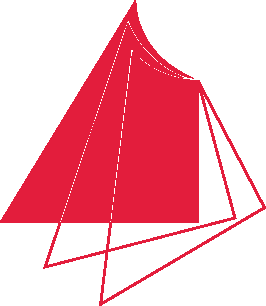
\includegraphics[width=0.25\textwidth]{hska}}


%% You can redefine the submission text:
% Default as per the University guidelines: This dissertation is submitted for
% the degree of Doctor of Philosophy
\renewcommand{\submissiontext}{Das inoffizielle Skript zur Informatik I Vorlesung}

%% Full title of the Degree 
\degree{geschrieben von Tobias Kerst}
 

%% Submission date
\degreedate{2014} 




% ***************************** Abstract Separate ****************************** 
% To printout only the titlepage and the abstract with the PhD title and the 
% author name for submission to the Student Registry, use the `abstract' option in
% the document class. 

\ifdefineAbstract
 \pagestyle{empty}
 \includeonly{Declaration/declaration, Abstract/abstract} 
\fi

% ***************************** Chapter Mode ***********************************
% The chapter mode allows user to only print particular chapters with references
% Title, Contents, Frontmatter are disabled by default
% Useful option to review a particular chapter or to send it to supervisior.
% To use choose `chapter' option in the document class

\ifdefineChapter
 \includeonly{Chapter3/chapter3} 
\fi

\setcounter{tocdepth}{1}

% ******************************** Front Matter ********************************
\begin{document}

\frontmatter

\begin{titlepage}

\maketitle

\end{titlepage}


% ******************************* Thesis Declaration ********************************

\begin{declaration}

Dieses Skript wurde erstellt, da eine vernünftige Zusammenfassung zur Informatik I Vorlesung an der Hochschule Karlsruhe zum Zeitpunkt dieser Ausarbeitung nicht vorlag. Das Ziel dieses Skripts ist es, eine grobe Zusammenfassung der am Anfang besprochenen Inhalte zu geben und Studenten das Lernen auf die Prüfung zu vereinfachen. 

Das Skript besteht aus drei Teilen. Der erste Teil beschäftigt sich mit den grundlegenden Datentypen, mit der internen Verwaltung von gewissen Datentypen bei Java und der Umrechnung verschiedener Zahlensysteme. Dieser Teil wurde anhand der in der Vorlesung besprochenen Verfahren zusammengeschrieben.

Der zweite Teil ist eine Zusammenfassung der Programmierkonventionen in der Programmiersprache Java. Der Inhalt ist von der Webseite \url{http://www.home.hs-karlsruhe.de/~pach0003/informatik_1/java_richtlinien/einleitung.html#uebersicht} genommen, welche von Prof. Dr. Pape angefertigt wurde. 

Der dritte Teil behandelt die Speicherverwaltung mittels Heap und Stack und die Modellierungsmöglichkeiten anhand der von UML zur Verfügung gestellten Aktivitäts- und Klassendiagramme. Hierzu wurden primär andere Quellen als Basis genommen, da die in der Vorlesung vorgestellten Konzepte sehr kurz gefasst wurden.

Dieses Skript ist ausschließlich zur privaten Nutzung gedacht, die Korrektheit der hier aufgeführten Informationen kann nicht gewährleistet werden. Solltest Du Fehler finden, werde ich diese gerne korrigieren.
Ich hoffe, dass Dir dieses Skript beim Lernen für die Klausur hilft.
% Author and date will be inserted automatically from thesis.tex \author \degreedate

\end{declaration}



% *********************** Adding TOC and List of Figures ***********************

\tableofcontents

% ******************************** Main Matter *********************************
\mainmatter

%*****************************************************************************************
%*********************************** First Chapter ***************************************
%*****************************************************************************************

\chapter{Datentypen und Zahlensysteme}  %Title of the First Chapter

\ifpdf
    \graphicspath{{Chapter1/Figs/Raster/}{Chapter1/Figs/PDF/}{Chapter1/Figs/}}
\else
    \graphicspath{{Chapter1/Figs/Vector/}{Chapter1/Figs/}}
\fi


%********************************** %First Section  **************************************
\section{Einführung} %Section - 1.1 

Am Anfang dieses Skriptes stehen die verschiedenen Datentypen, die es in Java (und vielen anderen Programmiersprachen) gibt. Auch werden wir uns angucken, was Dual-, Dezimal und Hexadezimalzahlen sind und wie man diese ineinander umrechnen kann. Außerdem wird noch beleuchtet, wie Java negative Zahlen im Speicher repräsentiert und was es mit der \textit{IEEE 754-Norm} auf sich hat.


\section{Datentypen}


Wenn man in Java programmiert, werden Konstanten und andere Werte in Variablen gespeichert, sodass man diese Werte später besser referenzieren kann. Diese Konstanten bezeichnet man heutzutage als \texttt{Literal}. Der \texttt{Datentyp} hingegen ist der Typ der Variable. Auf die Unterschiede dieser Datentypen gehen wir nun genauer ein. Am Ende der Ausführungen findet sich eine tabellarische Übersicht über die verschiedenen Datentypen, deren Literale und wie viel Platz diese im Speicher belegen.

\subsection{Bool'sche-Literale}

Es ist ein elementarer Bestandteil einer Programmiersprache, zu gucken, ob eine Aussage wahr oder falsch ist. Hierzu gibt es in Java den bool'schen Datentyp \texttt{Boolean}, der lediglich die Werte \textit{true} und \textit{false} annehmen kann. Anders als man das eventuell aus C++ kennt, existiert keine numerische Entsprechung, man kann also nicht false mit 0 gleichsetzen, oder irgendeinem anderen Wert.

\subsection{Integer-Literale}

Wenn man ganze Zahlen darstellen möchte, nutzt man hierzu für gewöhnlich das \texttt{Integer} Literal. Dieses kann Werte von etwa -2.000.000.000 (Milliarde) bis 2.000.000.000 darstellen. Genaueres kann man der Tabelle weiter unten entnehmen, welche die Wertebereiche und Größe etwas genauer darstellt. In Java kann man auch Integer-Literale dazu benutzen um Oktal-, oder Hexadezimalzahlen darzustellen. Im späteren wird darauf eingegangen, was das für Zahlen sind und wie man diese umrechnet. Für gewöhnlich reichen Integer Literale aus, um ganze Zahlen darzustellen. Für den Fall, dass der Platz nicht ausreicht, kann man auch auf das Long Literal zurückgreifen.

\subsection{Long-Literal}

Das \textbf{Long} Literal kann genau so wie das Integer Literal für ganze Zahlen benutzt werden, jedoch kann man im Long Literal größere Zahlen speichern, da dieses anstatt der 32 Bit, 64 Bit im Speicher einnimmt. Es wird aber dazu geraten, wenn nicht unbedingt nötig, ganze Zahlen als Integer zu speichern. Eine Besonderheit der Long Literale ist, dass diese ein \textit{L}, oder \textit{l} als Suffix haben. Möchte ich also den Wert $12$ als Long Variable speichern, so schreibe ich \texttt{long variablenName = 12L}.

\subsection{Gleitkomma-Literale}

Es gibt zwei Möglichkeiten, Gleitkommazahlen darzustellen. Die normale Schreibweise und die wissenschaftliche. Die normale Schreibweie besteht aus einer ganzen Zahl, welche durch einen \textit{.} von dem Bruchteil getrennt wird, bsp. $42.24$, $3.1415$. \underline{Wichtig}: Man benutzt nach amerikanischem Vorbild einen Punkt und kein Komma. 

Die wisenschaftliche Schreibweise, welche man im englischen auch als \textit{Exponential Notation} bezeichnet, bildet man, indem man eine Gleitkommazahl schreibt und an diese ein \textit{e}, oder \textit{E} anhängt, welches die Zehnerpotenz angibt. Man kennt e ja auch als Basis des natürlichen Logarithmus, das ist hier \textit{nicht} der Fall, in Java beschreibt \textit{E} einen Exponenten zur Basis 10. Mit dieser Schreibweise kann man sehr große, oder sehr kleine Zahlen sehr schön darstellen. Möchte ich nun $876.000.000$ darstellen, so kann ich auch $8.76E8$ schreiben. Aber auch $0.0000000987$ lässt sich schöner als $9.87E-8$ darstellen.

Es gibt in Java zwei Datentypen, die man verwenden kann. Zum einen das \texttt{Float} Literal, welches 32 Bit groß ist, als auch das \texttt{Double} Literal (64 Bit). Um das Float Literal zu nutzen, schreiben wir die Gleitkommazahl, wie gerade beschrieben, und hängen als Suffix ein \textit{F}, oder \textit{f} an. Somit kann man dann $42.24F$ (normale Schreibweise), oder aber $4.224E1f$ (wissenschaftliche Schreibweise) schreiben.

Wenn man das Suffix nicht an die Gleitkommazahl anhängt, konvertiert Java diese automatisch in ein Literal vom Typ \texttt{Double}, da dieses ohne Suffix auskommt. Somit sind die Zahlen $42.24$ und $4.224E1$ vom Typ Double. Wir benutzen in der Regel Literale vom Typ Double.

\subsection{Zeichen-Literale}

Möchte man ein einzelnen Zeichen speichern, so setzt man dieses in einfache Anführungszeichen, welches man als \texttt{Char} Literal bezeichet. Solche Zeichen können beispielsweise \textit{'§'}, \textit{'z'}, oder \textit{'T'} sein. Leider kann man über diese Methode nicht alle Zeichen angeben, da manche Zeichen eine besondere Funktion haben. \textit{'\textbackslash n'} ist zum Beispiel ein Symbol, welches eine Neue Zeile ausgibt, \textit{'\textbackslash t'} einen Tabulator. Und wenn man nun den Backslash in einem Zeichen Literal speichern möchte, hat man das Problem, dass dieses ja für die eben genannten Sonderzeichen benutzt. Deswegen ist für gewisse Zeichen eine sog. Escape-Sequenz nötig. \textit{'\textbackslash \textbackslash'} speichert also den Wert \textit{'\textbackslash'}.

Es ist zudem möglich, mit dem Escapezeichen \textit{\textbackslash} beliebige Zeichen des Unicode Zeichensatzes darzustellen, indem man eine besondere Schreibweise benutzt. \textit{'\textbackslash u0092'} steht für den Buchstaben \textit{e}.

\subsection{String-Literale}

String Literale werden anders als die Zeichen-Literale mit doppelten Anführungszeichen angegeben und können mehrere Zeichen beinhalten. Dies ist sinnvoll, wenn man eine Nachricht ausgeben möchte, den Namen eine Person speichern möchte, oder alles, was sonst mit Text zu tun hat. Auch hier kann man Zeilenumbrüche durch ein \textit{\textbackslash n} hervorrufen, als Beispiel soll die Floskel \textit{"Hallo \textbackslash n Welt"} dienen.
Es ist wichtig, vor allem wenn man das Thema Heap und Stack betrachtet, dass Strings keine primitiven Datentypen sind, sondern intern auch wie Objekte behandelt werden. Somit kann man auch auf den Strings Methoden aufrufen. Jedoch folgen Strings nicht der üblichen Syntax, die benutzt wird um Objekte zu initalisieren. Einen String initialisiert man wie folgt.

\begin{lstlisting}
String helloWorld = "Hello World";
\end{lstlisting}

\subsection{Zusammenfassung}

Wie man sieht, gibt es viele unterschiedliche Datentypen. Es handelt sich bei den hier behandelten Datentypen um sog. \textbf{primitive Datentypen} (\texttt{Strings} sind hier, wie gerade besprochen ausgenommen). Das bedeutet, dass diese nur einen gewissen Wertebereich aufnehmen können. Sie besitzen eine festgelegte Anzahl von Werten, was auch als \textit{Diskretheit} bezeichnet wird, aber auch eine feste Ober- und Untergrenze, wie man in der Tabelle $1.1$ erkennen kann. 

Außerdem ist es wichtig, dass man sich den begrenzten Speicherplatz bewusst macht. Das ist der Grund dafür, dass man reele Zahlen lediglich als gerundete Gleitkommazahl darstellen kann, worunter die Genauigkeit dann entsprechend leidet.

\begin{table}[ht] 
\caption{Die verschiedenen Datentypen in Java} 
\centering 
\begin{tabular}{l r r r r} 
\hline\hline 
Name & kleinster Wert & größter Wert & Größe in Bit & Literale\\ [0.5ex]  
\hline 
byte & -128 & 127 & 8 & 12\\
short & -32.768 & 32767 & 16 & 12\\
int & -2.147.483.648 & 2.147.483.647 & 32 & 12\\
long & $-9.2E^{18}$ & $9.2E^{18}$ & 64 & 12L\\
char & \textbackslash u0000 & \textbackslash uFFFF & 16 (Unicode) & 'a'\\
boolean & true, false & & 1 & true, false\\
float & $-1.4E^{45}$  & $3.4E^{38}$ & 32 (IEEE 754) & 1.2F\\
double & $-4.9E^{324}$ & $1.7E^{308}$ & 64 (IEEE 754) & 1.2\\
\hline 
\end{tabular} 
\label{table:nonlin} 
\end{table}


%********************************** 
%Zahlensysteme  
%**********************************


\section{Zahlensysteme} 

Die uns bekannten Zahlen sind die Dezimalzahlen und wie man an dem Teilwort {\em Dezi} erkennt, haben diese die Basis 10. Man kann die Zahl 53 also wie folgt darstellen 


$$53_{10} = 5 \cdot 10^{1} + 3 \cdot 10^{0}$$

Man kann aber nicht nur die natürlichen Zahlen darstellen, sondern auch Nachkommestellen und negative Zahlen sind möglich. Für die Nachkommastellen nimmt man einen negativen Exponenten, für negative Zahlen wird für gewöhnlich ein Vorzeichenbit gesetzt, das werden wir im späteren Verlauf kennen lernen. Gucken wir uns zunächst an, wie man Nachkommastellen bestimmen kann.

$$17,53_{10} = 1 \cdot 10^{1} + 7 \cdot 10^{0} + 5 \cdot 10^{-1} + 3 \cdot 10^{-2}$$

Jetzt möchten wir aber einen Schritt weiter gehen und eine Binärzahl, also eine Zahl mit der Basis 2, in eine Dezimalzahl (Basis 10) umwandeln.

\begin{eqnarray}
1101_{2} & = & 1 \cdot 2^{3} + 1 \cdot 2^{2} + 0 \cdot 2^{1} + 1 \cdot 2^{0} \\
& = & 1 \cdot 8 + 1 \cdot 4 + 0 \cdot 2 + 1 \cdot 1 \\
& = & 13_{10}
\end{eqnarray}

Nach diesem Vorbild kann man Zahlen auch im Oktalsystem (Basis 8) und Hexadezimalsystem (Basis 16) darstellen.

\begin{eqnarray}
275_{8} & = & 2 \cdot 8^{2} + 7 \cdot 8^{1} + 5 \cdot 8^{0} \\
& = & 128 + 56 + 5 \\
& = & 189_{10}
\end{eqnarray}
\begin{eqnarray}
10F_{16} & = & 1 \cdot 16^{2} + 0 \cdot 16^{1} + 15 \cdot 16^{0} \\
& = & 256 + 0 + 15 \\ 
& = & 271_{10}
\end{eqnarray}

\subsection{Dezimalzahlen}

\begin{itemize}
\item Folge der Ziffern 0 bis 9
\item keine führende 0
\item Vorzeichen möglich
\end{itemize}

Beispiel: 234, -23, 0 usw.

\subsection{Hexadezimalzahlen}

\begin{itemize}
\item Folge von 0 bis F (F$_{16} = 15_{10}$)
\end{itemize}

Beispiel: 011F, FFFA

\subsection{Oktalzahlen}

\begin{itemize}
\item Beginnen immer mit einer 0
\item Folge von 0 bis 7
\end{itemize}

Beispiel: 0117, 0771

\subsection{Umrechnung vom Dezimalsystem in Basis $b$}

Man kann vom Dezimalsystem sehr einfach in ein anderes Zahlensystem umwandeln, indem man eine Dezimalzahl ganzzahlig durch b teilt. Der Rest gibt dann den Wert im Zielsystem an. Diesen Schritt wiederholt man so oft, bis der ganzzahlige Anteil 0 übrig bleibt. Folgendes Beispiel gibt Auffschluss über diese Rechnung:

Basis $b = 8$
\begin{eqnarray}
97_{10} = 97 : 8 & = & \quad\text{12 Rest 1}\\
12 : 8 & = & \quad\text{1 Rest 4}\\
1 : 8 & = & \quad\text{0 Rest 1}
\end{eqnarray}

Ergebnis: $97_{10} = 141_{8}$

Das Ergebnis besteht aus den Restteilen, von unten nach oben gelesen. 

\subsection{Binärdarstellung}

Die maximale Anzahl der Binärstellen bei einem int sind 32 Stellen (32 Bit), bei long sind es 64 Stellen (64 Bit). Die Zahl wird von hinten aufgefüllt und falls vorne noch Zeichen frei stehen, werden diese mit einer 0 aufgefüllt. Nehmen wir beispielsweise die Zahl $15_{10}$, deren Binärdarstellung ja $1111_{2}$ ist, so wird diese Zahl im Speicher als 00\dots0001111. Eine weitere Besonderheit, die vorher bereits schon einmal angesprochen wurde, ist die Darstellung der negativen Zahlen. Möchten wir eine negative Zahl schreiben, beispielsweise $-15_{10}$, so wird diese Zahl als 100\dots0001111 gespeichert. Es gibt jedoch ein besseres Verfahren um negative Zahlen zu speichern und zwar das 2er Komplement.

\section{Das 2er Komplement}

\subsection{Von der Dezimalzahl zum 2er Komplement}

Java benutzt die 2er Komplement Codierung, um negative Zahlen zu speichern. Dies ist sinnvoll, da kein Platz für $+$ und $-$ verschwendet werden muss. Zuerst wird das Vorzeichen abgetrennt und die Zahl im Dualsystem dargestellt, so wie wir das bisher gemacht haben. Im Anschluss wird das Komplement gebildet. Wir beenden das Ganze, indem wir noch 1 hinzuaddieren. Anschaulicher wird dies, wenn wir uns folgendes Beispiel angucken.

\begin{eqnarray} \label{2er Komplement bilden}
-89_{10} & \Rightarrow & 0101\ 1001 \\
& \Rightarrow & 1010\ 0110 \quad\text{(Komplement bilden)}\\
& \Rightarrow & 1010\ 0111 \quad\text{(1 hinzu addieren)}
\end{eqnarray}

Zu beachten ist, dass das Vorzeichen am Anfang erst einmal ignoriert wird. Dann wird einfach jedes Zeichen umgedreht (also das Komplement gebildet) und wie bereits beschrieben wird 1 hinzuaddiert. Außerdem gilt es zu beachten, dass der Wertebereicht für ein 8-Bit 2er Komplement von $-128$ bis $127$ geht. Angenommen man addiert $127 + 1$, dann springt der Wert zu $-128$. Dies ist eine Form des ungewollten Überlaufs.

\subsection{Vom 2er Komplement zur Dezimalzahl}

Die 2er-Komplementdarstellung eignet sich erstklassig, um schnell sagen zu können, ob eine Zahl positiv, oder negativ ist. Ein Blick auf das erste Bit gibt uns darüber eine Auskunft, wie wir die Zahl lesen müssen. Ist es eine $0$, so können wir die Zahl nach unserem bereits bekannten Schema einfach in eine Dezimalzahl umwandeln. Ist es eine $1$, die Zahl also negativ, so gilt es diese wie folgt umzuwandeln.  

\begin{eqnarray}
1010\ 0111_{2} & \Rightarrow & \ 0101\ 1000 \quad\text{(Komplement bilden)}\\
& \Rightarrow & \ 0101\ 1001 \quad\text{(1 hinzu addieren)}\\
& \Rightarrow & -89_{10} \quad\text{(Dezimalzahl bilden und Vorzeichen anhängen)}
\end{eqnarray}


\section{IEEE 754}

\subsection{Gleitkommazahlen}

Gleitkommazahlen können sehr unterschiedlich große Zahlen darstellen. So kann man riesig große Zahlen ($1,23\cdot 10^{88}$) darstellen, aber auch winzig kleine ($1,23\cdot 10^{-88}$) und Selbiges gilt auch für den negativen Bereich. Wie man bereits an der Notation sieht, die genutzt wird um diese riesigen Zahlenbereiche abzudecken, lohnt es sich, hier die wissenschaftliche Schreibweise zu nutzen, um Zahlen darzustellen. Um im Folgenden sprachliche Barrieren zu vermeiden möchte ich an dieser Stelle auf die verschiedenen Bezeichnungen der einzelnen Teile in der wissenschaftlichen Schreibweise eingehen.

$$ x = v \cdot m \cdot b^{e}$$

\begin{itemize}
\item \textbf{v} ist das Vorzeichen
\item \textbf{m} ist die Mantisse
\item \textbf{b} ist die Basis (bei IEEE 754 \textit{b = 2})
\item \textbf{e} ist der Exponent
\end{itemize}

Für das Vorzeichen $v$ gilt im Folgenden, dass dieses aus einem Bit besteht und $0$ für ein positives und $1$ für ein negatives Vorzeichen steht. Man kann auch sagen, dass $ v = (-1)^{v} $ repräsentiert. Es ist aber einfacher sich einfach zu merken, dass das gesetzte Bit ($= 1$) eine negative Zahl repräsentiert

Diese etwas ungewohnte Art der Darstellung soll an den folgenden beiden Beispielen deutlich werden.

\begin{eqnarray}
-543,21 & = & (-1)^{1} \cdot 5,4321 \cdot 10^2 \\
0,00543 & = & 1 \cdot 5,4321 \cdot 10^{-3}
\end{eqnarray}


Wir müssen beachten, dass Gleitkommazahlen oft nur einen angenäherten Wert annehmen können, da reele Zahlen beispielsweise nicht in den Speicher passen (mit ihren unendlich vielen Nachkommastellen), aber auch Rundungsfehler das Arbeiten mit Gleitkommazahlen erschweren. Wie die Gleitkommazahlen in Computern dargestellt werden und was das alles mit diesem \textit{IEEE 754} zu tun hat, wird in den folgenden Abschnitten erklärt.

\subsection{Was ist das und warum wird es genutzt}

Die IEEE 754 Norm wird genutzt um Gleitkommazahlen in Computern darzustellen und diese umzurechnen, aber auch, wie man mathematische Operationen mit diesen Zahlen durchführt und wie diese Zahlen zu runden sind. Es wird generell zwischen Datenformaten mit 32 Bit (\textit{single precision}) und 64 Bit (\textit{double precision}) Speicherbedarf unterschieden. Java nutzt \texttt{Float} für die Single-Precision Darstellung, und \texttt{Double} für die Double Precision. 

Die Single Precision Zahl benötigt den folgenden Speicherplatz für die einzelnen Teile, die zur Darstellung einer Gleitkommazahl notwendig sind

\begin{itemize}
\item Vorzeichen: 1 Bit
\item Exponent: 8 Bit
\item Mantisse: 23 Bit
\end{itemize}

Die Anordnung der verschiedenen Bits soll durch folgende Abbildung besser erklärt werden.

\begin{figure}[htbp!] 
\centering    

\includegraphics[width=1.0\textwidth]{ieee}
\label{fig:ieee}
\end{figure}

Die Double Precision Zahl benötigt hingegen folgenden Speicherplatz

\begin{itemize}
\item Vorzeichen: 1 Bit
\item Exponent: 11 Bit
\item Mantisse: 52 Bit
\end{itemize}

Die Mantisse wird bei der IEEE Kodierung im Bereich $ 1 \le m \le 2 $ dargestellt. Da dann links immer eine 1 steht, vor dem Komma, müssen wir dieses nicht extra speichern und erhalten somit 1 Bit mehr Platz für die Mantisse.

Außerdem können noch einige Sonderfälle auftreten, die durch spezielle Bitmuster kodiert werden. Hierzu werden zwei besondere Exponentwerte benutzt, der Maximalwert ($e = 111\dots11 = 2^{r} - 1$) und die Null ($e = 000\dots00$). Mit dem maximalen Exponentwerten werden die Sonderfälle \textit{NaN} (Englisch für \textit{Not a Number}) und $\infty$ kodiert. Mit der Null im Exponenten wird die Gleitkommazahl 0 dargestellt.

Jetzt, wo wir grob wissen, was es mit der IEEE 754 Norm auf sich hat, möchten wir uns einmal angucken, wie wir eine Dezimalzahl in eine solche IEEE 754 normierte single precision Zahl umwandeln.


\subsection{Dezimalzahl in IEEE 754 umrechnen}

Wir möchten das Umrechnen von einer Gleitkommazahl in eine IEEE 754 normierte Binärzahl am Beispiel von $-10,125$ erklären.

\subsubsection{Vorzeichen}

Da unsere Beispielzahl $-10,125$ negativ ist, setzen wir das Vorzeichenbit auf 1 und entfernen das Vorzeichen von der Zahl, sodass wir von nun an mit $10,125$ weiterrechnen werden.

\subsubsection{In Binärzahl umwandeln}

Nun wandeln wir $10,125$ in eine Binärzahl um.

\begin{eqnarray}
10,125_{10} & = & 1 \cdot 8 + 0 \cdot 4 + 1 \cdot 2 + 0 \cdot 1 + 0 \cdot 0.5 + 0 \cdot 0.25 + 1 \cdot 0.125 \\
& = & 2^{3} + 2^{1} + 2^{-3} \\
& = & 1010,001_{2}
\end{eqnarray}

\subsubsection{Mantisse bilden, Exponent bestimmen}

Nun, da wir die Binärzahl $1010,001_{2}$ haben, bilden wir daraus die Mantisse und können danach den Exponenten bestimmen. Zuerst verschieben wir das Komma so, dass nur noch eine 1 vor dem Komma steht.

$$1010,001 = 1,010001 \cdot 2^{3}$$

Die Mantisse erhalten wir, wenn wir nun die vor dem Komma stehende 1 abtrennen und die hinteren Bits mit Nullen auffüllen (die Mantisse besteht ja bei der single precision aus 23 Bits). Somit erhalten wir folgende Mantisse:

$$0100010000\ 00000000000\ 000$$

Jetzt fehlt uns nur noch der Exponent. Den erhalten wir, wenn wir den Term von oben betrachten, in dem wir das Komma verschoben haben.

$$ 1,010001 \cdot 2^{3}$$

Hier erkennen wir, dass der Exponent $3$ ist. Nun müssen wir 127 mit diesem Exponenten addieren und die Summe nur noch in eine Binärzahl umwandeln:

$$127 + 3 = 130_{10} = 1000\ 0010_{2}$$

Nun haben wir die drei notwendigen Bestandteile

\begin{eqnarray}
Vorzeichen & & 1 \\
Exponent & & 1000\ 0010\\
Mantisse & & 0100010000\ 00000000000\ 000
\end{eqnarray}

aus denen wir nun die der IEEE 754 Norm entsprechende 32 Bit Gleitkommazahl zusammen fassen können

$$\underbrace{1}_{VZ}\underbrace{10000010}_{Exponent}\underbrace{010001000000000000000000}_{Mantisse}$$

\subsection{IEEE 754 Zahl in Dezimalzahl umwandeln}

Auch hier ist es einfacher, die Umformung anhand eines Beispiels zu zeigen. Nehmen wir die als IEEE 754 normierte Binärzahl $1\ 011111110\ 01101100$, bei der wir die letzten Füllbits (also Nullen) weglassen.

An dem Vorzeichenbit $1$ erkennen wir bereits, dass es sich um eine negative Zahl handelt. Nun gucken wir, wie groß der Exponent ist und in welche Richtung sich das Komma demzufolge verschieben wird. Dazu berechnen wir zuerst die Dezimaldarstellung.

$$01111\ 1110_{2} = 126_{10}$$

Und ziehen hiervon 127 ab.

$$126 - 127 = -1$$

Das Komma verschiebt sich also nach links, die Zahl ist somit kleiner als 1. Wir nehmen nun wieder die Mantisse, fügen vorne eine 1 und folgend das Komma an und verschieben über den gerade berechneten Exponenten das Komma. Danach berechnen wir aus dieser Dualzahl die Dezimalzahl

\begin{eqnarray}
1,\underbrace{01101100}_{Mantisse} \cdot 2^{\overbrace{-1}^{Exponent}} & = & 0,101101100\\
& = & 0 \cdot 2^{0} + 1 \cdot 2^{-1} + 0 \cdot 2^{-2} + 1 \cdot 2^{-3}\\
& & + 1 \cdot 2^{-4} + 0 \cdot 2^{-5} + 1 \cdot 2^{-6} + 1 \cdot 2^{-7}\\
& = & 2^{-1} + 2^{-3} + 2^{-4} + 2^{-6} + 2^{-7}\\
& = & 0.7109375_{10}
\end{eqnarray}

Wenn wir nun noch das Vorzeichen beachten, welches ja eine negative Zahl forderte, erhalten wir die Dezimalzahl

$$- 0.7109375$$

\subsection{Nachkommastellen von Dualzahlen berechnen}

Es gibt eine einfache Möglichkeit die Nachkommastellen von Dualzahlen zu berechnen. Auch an dieser Stelle ist ein Beispiel die beste Möglichkeit, das Verfahren zu verstehen. Wir wollen $0.625$ als Dualzahl darstellen. Dies geht wie folgt:

\begin{eqnarray}
0,625 \cdot 2 = 1,25 & | & \to 1\\
0,25 \cdot 2 = 0,5 & | & \to 0\\
0,5 \cdot 2 = 1 & | & \to 1\\
& \Rightarrow & 0,101_{2}
\end{eqnarray}

Dies ist ein relativ einfaches Beispiel. Gucken wir uns nun an, wie wir die Zahl $0,4$ (näherungsweise berechnen können)

\begin{eqnarray}
0,4 \cdot 2 = 0,8 & | & \to 0\\
0,8 \cdot 2 = 1,6 & | & \to 1\\
0,6 \cdot 2 = 1,2 & | & \to 1\\
0,2 \cdot 2 = 0,4 & | & \to 0
\end{eqnarray}

Wie man erkennt, wiederholt sich diese Folge, da man wieder bei $0,4$ auskommt. Es entsteht also die Binärzahl

$$0,0110\ 0110 \dots$$

\section{Overflow}

Wenn man in Java programmiert, muss man bei einigen Datentypen aufpassen, dass man keinen Overflow, oder aber Underflow erreicht. Wir haben ja bereits die Wertebereiche der verschiedenen Datentypen angeguckt. Dies ist vor allem gefährlich, da Java keine Exception schmeißt, sollte man den Wertebereich übertreten. Wählt man den größten positiven Wert (011111\dots11$_{2}$) einer Zahl und addiert eine 1 hinzu, wird dieser zu 100000\dots und somit zur kleinsten negativen Zahl. Nehmen wir der Einfachheit halber den Byte Datentyp, der von -128 bis 127 reicht.

\begin{lstlisting}
byte b = 128; // Fehler, weil 127 der größte Wert ist
byte b = 127; //richtig

// Wenn man 1 addiert, erreicht man einen overflow
byte b = b + 1; // b = -128;

byte b = -128;
byte b = b - 3; // b = 125
\end{lstlisting}

Wie man sieht, bekommt man Werte, die man eventuell nicht erwartet hat. Man sollte deswegen in seine Programme Kontrollmechanismen einbauen, die die Operationen im vorhinein prüfen, sollte man ein solches Verhalten nicht wünschen.
%*****************************************************************************************
%*********************************** Second Chapter **************************************
%*****************************************************************************************

\chapter{Java Konventionen}

\ifpdf
    \graphicspath{{Chapter2/Figs/Raster/}{Chapter2/Figs/PDF/}{Chapter2/Figs/}}
\else
    \graphicspath{{Chapter2/Figs/Vector/}{Chapter2/Figs/}}
\fi

Java ist eine Hochsprache. Das heißt, dass die Sprache abstrakt ist und als solche nicht direkt von der Maschine gelesen werden kann. Hierzu ist ein sog. Compiler nötig, der aus der Hochsprache ausführbare Programme erstellt. Wenn man ein Javaprogramm schreiben will, kommt der Quellcode, also die Programmanweisungen in eine Quelldatei, welche mit .java endet. Diese wird dann vom javac Compiler in eine .class Datei umgewandelt. Diese Datei kann dann im Anschluss von dem Java Interpreter, der Java Virtual Machine gelesen und ausgeführt werden.
Programme bestehen aus Symbolen, die alle eine eigene Bedeutung, oder Funktion haben
\begin{itemize}
\item Schlüsselwörter: public, class, static, double
\item Bezeichner: gewicht, BodyMassIndex usw.
\item Literale: 1.82, 182736292L, "Hallo Welt"
\item Trennsymole: {}, [], =, *, +, -, / usw.

Um den Code auch für Menschen gut lesbar zu machen, ist es nötig, einheitlichen Code zu schreiben, also den Programmcode immer nach dem selben Schema zu schreiben und zu strukturieren. Es gilt somit, semantisch und syntaktisch korrekten Code zu schreiben. Hier ist der in der Vorlesung festgelegte Standard zusammengefasst.
\end{itemize}

\section{Syntax}
\subsection{Aussagekräftige Namen verwenden}

\paragraph{Regel:} Verwende für Bezeichner immer aussagekräftige und selbsterklärende Namen.
\paragraph{Regel:} Verwende keine Abkürzungen in Bezeichner – schreiben diese Namen immer aus.
\paragraph{Begründung:} Quelltexte werden dadurch für alle lesbarer und verständlicher.

\paragraph{Beispiel}
Statt \texttt{KFZ, BA, HS, DB} \ besser\  \texttt{Kraftfahrzeug, BundesagenturFuerArbeit, HochschuleKarlsruhe, DeutscheBahn} schreiben.

\subsection{Nur eine Sprache verwenden}

\paragraph{Regel:} Vermische keine verschiedenen Sprachen (Deutsch, Englisch, …) in einer Klasse
\paragraph{Begründung:} Quelltexte werden dadurch für alle lesbarer und verständlicher.

\subsection{Nur alphanumerische Zeichen verwenden}

\paragraph{Regel:} Vermische keine verschiedenen Sprachen (Deutsch, Englisch, …) in einer Klasse
\paragraph{Begründung:} Quelltexte werden dadurch für alle lesbarer und verständlicher.

\paragraph{Beispiel}
\texttt{Person, zugFahren, ueberpruefen, MAXIMALE\textunderscore\text{ANZAHL}}

\subsection{Verwende Upper Case Camel Style}

\paragraph{Regel:} Bei Bezeichner, die aus mehreren Teilwörtern bestehen, wird der erste Buchstabe jedes Teilworts (ab dem zweiten Teilwort) groß geschrieben, wenn die entsprechenden Wörter normal auseinander geschrieben würden.
\paragraph{Begründung:} Damit lange Bezeichner lesbarer sind.

\paragraph{Beispiel}
\texttt{zugFahren, Donaudampfschifffahrt, HochschuleKarlsruhe}

\section{Variablen}

\subsection{Anfangsbuchstabe kleinschreiben}

\paragraph{Regel:} Schreibe Variablen klein (Ausnahme sind Konstanten). Besteht eine Variable aus mehren Teilwörtern, so wird bei jedem folgenden Teilwort der erste Buchstabe groß geschrieben.
\paragraph{Begründung:} Ein Bezeichner ist dadurch im Quelltext sofort als Variable erkennbar.

\paragraph{Beispiel}
\texttt{manfredMueller, anzahlPersonen, quersumme}

\subsection{Konstanten mit Grossbuchstaben schreiben}

\paragraph{Regel:} Konstanten (static final) werden immer mit Grossbuchstaben bezeichnet und Teilwörter mit dem Unterstrich \textunderscore abgetrennt.
\paragraph{Begründung:} Ein Bezeichner ist dadurch im Quelltext sofort als Konstante erkennbar.

\subsection{Zählvariablen}

\paragraph{Regel:} Verwende die Buchstaben \texttt{i, j, k, l} für rein technische ganzzahlige Schleifenvariablen.
\paragraph{Begründung:} Aus historischen Gründen.

\begin{lstlisting}
for (int i = 0; i < personen.length; i++) {
   ... 
} 
\end{lstlisting}

Für die Aufzählung aller Elemente eines Feldes oder einer Datenstruktur des Java Collection Frameworks, sollte aber möglichst die ab JDK 5.0 zusätzliche for-Schleife verwendet werden. Die technischen Schleifenvariablen werden dann ganz vermieden:

\begin{lstlisting}
for (Person person : personen) {
  ...
}
\end{lstlisting}

\subsection{this Objektattributen voranstellen}

\paragraph{Regel:} Um besser zwischen Objektattribute und lokalen Variablen zu unterscheiden, sollten Objektattribute mit this referenziert werden.
\paragraph{Begründung:} Die Quelltexte werden lesbarer und Fehler werden vermieden.

\paragraph{Beispiel} \hspace{0pt}\\
\begin{lstlisting}
this.name = name; // wobei name ein Parameter ist
\end{lstlisting}


\subsection{Ungarische Notation vermeiden}

\paragraph{Regel:} Verwende keine Ungarische Notation.
\paragraph{Begründung:} Damit Quelltexte lesbarer und wartbarer werden.

Bei der Ungarischen Notation werden zwei Präfixe dem eigentlichen Bezeichner vorangestellt: Der erste für den Verwendungszweck des Bezeichners, der zweite für den Typ. Zum Beispiel p für Pointer, i für Integer: piAnzahl ist ein Zeiger auf einen Integerwert.


\section{Methoden}

\subsection{Verb verwenden}

\paragraph{Regel:} Verwende mindestens ein Verb in Präsensform für eine Methode. Das Verb soll möglichst genau beschreiben, was die Methode macht.
\paragraph{Begründung:} Damit Quelltexte verständlicher werden.

\paragraph{Beispiel}
\texttt{personSuchen(), loeschen(), produktVerkaufen()}

\subsection{Getter/Setter}

\paragraph{Regel:} Verwende als Verb das englische Präfix \texttt{get} mit einem nachfolgenden Substantiv, wenn eine Methode (ohne Parameter) einen Wert, der durch das Substantiv beschrieben ist, zurückgibt. Bei getter-Methoden mit booleschen Rückgabewert, wird statt get meist is verwendet.
\paragraph{Regel:} Verwende als Verb das englische Präfix \texttt{set} mit einem nachfolgenden Substantiv, wenn eine Methode ohne Rückgabewert und mit einem Parameter einen Zustandswert (insbesondere ein Attribut) eines Objekts ändert.
\paragraph{Begründung:} Zur Wahrung des Geheimnisprinzips bei der Programmierung.

\paragraph{Beispiel}
\texttt{String getVorname(), void setVorname(String vorname),\\boolean isSchaltjahr(), void setSchaltjahr(boolean schaltjahr)}

\section{Quelltextformatierung}

\subsection{Programmierstile}

\paragraph{Regel:} Mische in einer Klasse nie verschiedene Programmierstile.
\paragraph{Regel:} Bei bestehenden Quelltexten gilt insbesondere, dass der bestehende Programmierstil übernommen oder überall in der Klasse geändert wird.
\paragraph{Begründung:} Quelltexte werden dadurch für alle lesbarer.

\subsection{Allgemeine Regel}

\paragraph{Regel:} Schreibe nie Zeilen mit mehr als 80 Zeichen.
\paragraph{Regel:} Stelle den Editor so ein, dass er diese Grenze als vertikale Linie klar darstellt.
\paragraph{Begründung:} Quelltexte werden dadurch lesbarer.

Die 80 Zeichengrenze hat historischen Gründe: frühe Terminals hatten max. 80 Zeichen pro Zeile. Heutzutage ist die Grenze je nach Bildschirmauflösung und Font etwas größer. Grundsätzlich sollte man aber nicht von einer zu hohen Anzahl Zeichen pro Zeile ausgehen. Überlange Zeilen sind für Menschen schlecht lesbar, da nur eine begrenzte Anzahl von „Wörtern“ (ca. 5-7) mühelos erfasst werden können ohne dass man das Gefühl bekommt angestrengt zu lesen. Des Weiteren ist das horizontale Scrollen bei überlangen Zeilen im Fenster im Gegensatz zum vertikalen mühsam, da bei Sprung auf die nächste Zeile, insgesamt der Quelltext sich sprunghaft nach links verschiebt (zu starker Kontextwechsel).

\subsection{Einrückungen}

\paragraph{Regel:} Verwende bei Kontrollstrukturen wie if, else, while, … immer geschweifte Klammer für die Anweisungen (auch bei Einzelanweisungen)
\paragraph{Regel:} Rücke jede Anweisung um 2 bis 4 Zeichen nach rechts ein (immer konsistent die gleiche Anzahl von Zeichen und nicht mal 2, mal 3 und dann mal wieder 4 Zeichen)
\paragraph{Regel:} Stelle den Editor so ein, dass bei Drücken der Tabulatortaste, immer Leerzeichen eingefügt werden.
\paragraph{Begründung:} Bessere Lesbarkeit von Programmen und vermeiden von Programmierfehlern.

\paragraph{Beispiel} \hspace{0pt}\\
\begin{lstlisting}
if (student.hatZulassung () && student.hatZugesagt()) {
  student.immatrikulieren();
}
\end{lstlisting}

Falls die Klammern bei einzelnen Anweisungen weggelassen werden, kann bei nachträglichem Hinzufügen von zusätzlichen Anweisungen oder anderen Änderungen vergessen werden, die Klammern zu setzten, da durch die Einrückung suggeriert wird, dass die Anweisungen zusammengehören.

Werden Tabulatore statt Leerzeichen im Quelltext eingefügt, dann geht aufgrund anderer Tabulatoreinstellungen bei einem anderen Editor die Struktur meist die Struktur verloren.

Wenn bei if und else Klammern weggelassen werden, dann gehört das else zum "nächsten" vorangehenden if. Dies kann zu ungewollten Fehlern führen. Im folgenden Beispiel scheint das else zum ersten if zu gehören, weil es nicht eingerückt ist. Tatsächlich gehört es zum zweiten if!!!

\paragraph{Beispiel} \hspace{0pt}\\
\begin{lstlisting}
if (  ) 
   if (   )
     ....
else 
  ....
\end{lstlisting}

Wenn immer Klammern verwendet werden, ist es für jeden Programmierer eindeutig, zu welchem if ein else gehört:

\begin{lstlisting}
if (  ) {
   if (   ) {
     ....
   }
} else { 
  ....
}
\end{lstlisting}

\subsection{else-if}

Ausnahme obiger Regel: Folgt auf \texttt{else} direkt wieder ein \texttt{if}, so braucht das if nicht in ein Paar geschweifter Klammern eingeschlossen zu werden.
\paragraph{Begründung:} Damit Quelltexte lesbarer werden.

\paragraph{Beispiel} \hspace{0pt}\\
\begin{lstlisting}
if (a < 7) {
   a = a + 1;
} else if (a > 10) {
   a = a - 1;
} else if (a == 1) {
   ...
}
\end{lstlisting}

Dies vermeidet, dass bei einem kaskadierenden if-else if-else if - … - else durch fortgesetztes Einrücken die Zeilen immer weiter nach rechts wandern und so der Quelltext unnötig tief verschachtelt ist. Man kann sich diese Regel auch so verstellen, dass damit im Gegensatz zu anderen Programmiersprachen ein in Java nicht vorhandenes Schlüsselwort „elsif“ simuliert wird.

\subsection{Klammerungsstil}

\paragraph{Regel:} Schreibe entweder \par\textit{a)} die geschweifte öffnende Klammer auf die nächste Zeile oder \par\textit{b)} hinter der Kontrollanweisung ohne weitere Anweisungen hinter der öffnenden Klammer. Schreibe die zugehörige schließende Klammer immer auf eine neue Zeile ohne weitere Anweisungen oder Bezeichner davor oder dahinter (Ausnahme else).
\paragraph{Begründung:} Damit Quelltexte kürzer und lesbarer werden.

\paragraph{Beispiel zu a)} \hspace{0pt}\\
\begin{lstlisting}
if (a > 7)
{
   a = a + 1;
}
\end{lstlisting}

\paragraph{Beispiel zu b)} \hspace{0pt}\\
\begin{lstlisting}
if (a > 7) {
   a = a + 1;
} else {
   a = a - 1;
}
\end{lstlisting}

\subsection{Eine Anweisung pro Zeile}

\paragraph{Regel:} Schreibe jede einzelne Anweisung in eine separate Zeile.
\paragraph{Begründung:} Damit Quelltexte lesbarer werden.

\subsection{Continue und Break vermeiden}

\paragraph{Regel:} Vermeide die Schlüsselwörter continue und break, um Schleifen fortzuführen oder eine Kontrollstruktur abzubrechen. Ausnahme: break bei case-Anweisungen.
\paragraph{Begründung:} Durch break und continue in Kontrollanweisungen wird der sequentielle Kontrollfluss unterbrochen. Dadurch ist dieser für Menschen nicht so leicht zu verstehen.

\subsection{Verschachtelungstiefe von Kontrollanweisungen}

\paragraph{Regel:} Vermeide eine zu tiefe Verschachtlung von Kontrollanweisungen (ca. drei Kontrollanweisungen).
\paragraph{Begründung:} Damit Quelltexte lesbarer werden.

\subsection{Leerzeichen bei Operatoren}

\paragraph{Regel:} Setzte vor und nach jedem binären Operator ein Leerzeichen.
\paragraph{Begründung:} Damit Ausdrücke bei langen Bezeichnern lesbarer werden.

\paragraph{Beispiel} \hspace{0pt}\\
\begin{lstlisting}
a = 1 + 7 * (5 / a);
flaecheninhalt = kreisradius * kreisradius * 3.14159265;
\end{lstlisting}

\subsection{Umbrechen von überlangen Ausdrücken}

\paragraph{Regel:} Breche überlange Zeilen wie folgt um:
\begin{itemize}
\item bei arithmetischen Operatoren vor einem Operator mit der schwächsten Bindung (Operatoren so auswählen, dass nicht zu viele Zeilenumbrüche entstehen)
\item bei Methodenaufruf oder Parameterdeklaration nach einem Komma
rücke den umgebrochenen Teil soweit nach rechts ein, dass er sich unterhalb des zugehörigen linken Teilausdrucks des Operators befindet mit zwei bis vier zusätzlichen Leerzeichen
\end{itemize}
\paragraph{Begründung:} Damit Quelltexte lesbarer werden.


\paragraph{Beispiel} \hspace{0pt}\\
\begin{lstlisting}
                           | <-- soll das Zeilenende markieren
a * a * a + 3 * a * a * b + 3 * a * b * b + b * b *b
\end{lstlisting}

Nicht bei *, sondern bei + umbrechen (+ bindet schwächer als *)

\begin{lstlisting}
a * a * a + 3 * a * a * b
     + 3 * a * b * b + b * b *b
\end{lstlisting}

\paragraph{Beispiel} \hspace{0pt}\\
\begin{lstlisting}
                                   |
x1 * 3 + (a + b + 6) * ((x2 + 8) + x3 / 11)
\end{lstlisting}

Bei + umbrechen im zweiten Faktor, wäre schlecht, da durch Einrücken, dann x3 / 11 über die Grenze hinausragt. Deswegen besser bei * umbrechen.

\begin{lstlisting}
x1 * 3 + (a + b + 6)
            * ((x2 + 8) + x3 / 11)
\end{lstlisting}


\paragraph{Beispiel} \hspace{0pt}\\
\begin{lstlisting}
public Address(String strasse,
                 String hausnummer,
                 int postleitzahl,
                 String ortsname) {
  ...
}
\end{lstlisting}

\subsection{Vergleich mit boolschen Werten}

\paragraph{Regel:} Vergleiche Boolesche Werte in einem Booleschen Ausdruck nicht mit == auf true oder false. Verwende stattdessen bei true, den Booleschen Ausdruck selbst und bei false dessen Negation (bei != entsprechend umgekehrt)
\paragraph{Begründung:} Quelltexte werden leserlicher


\paragraph{Beispiel}
Anstatt folgenden boolschen Ausdruck\par
\begin{lstlisting}
schaltjahr == true && volljaehrig == false
\end{lstlisting}

verwende besser

\begin{lstlisting}
schaltjahr && ! volljaehrig
\end{lstlisting}

\subsection{Operatorenreihenfolge}

\paragraph{Regel:} Bei mathematischen Vergleichen wie 0 < i < j < n behalte die Reihenfolge der Operatoren und Variablen in der Implementierung bei.
\paragraph{Begründung:} Der resultierende Ausdruck ist dann sehr nah an der mathematischen Schreibweise orientiert und leichter verständlich, da er die ursprüngliche zu implementierende Form beibehält.

\paragraph{Beispiel} \hspace{0pt}\\
\begin{lstlisting}
if (0 < i && i < j && j < n) {
   ...
}
\end{lstlisting}

Oder für $i = j = 7 < n$

\begin{lstlisting}
if (i == j && j == 7 && 7 < n) {
   ...
}
\end{lstlisting}

\subsection{Vermeide Seiteneffekte}

\paragraph{Regel:} Ein Ausdruck sollte keine Seiteneffekte haben, das heisst, ein Ausdruck sollte keine Zustandsänderungen durchführen.
\paragraph{Regel:} Insbesondere sollten Funktionen keine Seiteneffekte haben.
\paragraph{Begründung:} Vermeidung von Programmierfehlern und bessere Verständlichkeit von Quelltexten.

\paragraph{Beispiel} Welchen Wert hat a, nachdem die letzte Anweisung ausgeführt wurde? \par
\begin{lstlisting}
int a = 1;

a = (a = 2) + (a += a) * (a = 1 + a);
\end{lstlisting}

\subsection{Vermische Kurzschlußoperatoren nie mit "normalen" Booleschen Operatoren}

\paragraph{Regel:} Vermische nie die Kurzschlußoperatoren (\&\&,||) mit den "normalen" Booleschen Operatoren (\&, \string^, |) in einem Ausdruck
\paragraph{Begründung:} Fehlervermeidung und Wartbarkeit

\paragraph{Beispiel} Welchen Wert hat folgender Ausdruck?\par

\begin{lstlisting}
false && true | true
\end{lstlisting}

\&\& bindet \textbf{schwächer} als |. Deswegen ist der Wert des Ausdrucks false und nicht true, wie es \textit{logischerweise} sein müsste.

\subsection{Kurzer Methodenrumpf}

\paragraph{Regel:} Verwende nur so viele Zeilen für die Implementierung einer Methode, so dass die Methode komplett auf den Bildschirm passt (ca. 20-30 Zeilen), wenn möglich auch noch die zugehörige Javadokumentation.
\paragraph{Regel:} Verlagere bei zu langen Zeilen zusammengehörende Teile in private Methoden.
\paragraph{Begründung:} Um die Struktur und Funktionsweise einer Methode zu verstehen, sollte der Programmierer nicht gezwungen sein, vertikal zu scrollen: zugehörige Programmteile if-else sind dann oft nicht mehr auf einen Blick zu erfassen. Mit den Refactor-Funktionen der Entwicklungsumgebung geht eine derartige nachträgliche Formatierung des Quelltextes sehr schnell.

\subsection{Deklaration lokaler Variablen}

\paragraph{Regel:} Deklariere alle lokalen Variablen (außer Schleifenvariablen) am Anfang der Methode gefolgt von einer Leerzeile.
\paragraph{Regel:} Bei einer Funktion sollte insgesamt nur ein return in der Methode existieren (notwendigerweise am Ende der Methode). Setzte vor diesem return eine Leerzeile.
\paragraph{Begründung:} Damit Methodenimplementierung verständlicher wird.

\subsection{Primitive Datentypen}

\paragraph{Regel:} Verwende möglichst int statt byte, short oder long
\paragraph{Regel:} Verwende möglichst double statt float
\paragraph{Regel:} Mische möglichst keine verschiedenen Zahlentypen in einem Ausdruck.
\paragraph{Regel:} Verwende wissenschaftliche Notation nur bei sehr kleinen oder sehr großen Zahlen.

Byte und short haben im Gegensatz zu int und long einen relativ kleinen Wertebereich. Da ein Überlauf in Java anderes als in C\# nicht durch eine Ausnahme angezeigt wird, sollte möglichst mit Datentypen höherer Genauigkeit gerechnet werden. int ist meist ausreichend vom Wertebereich und schneller als long. Es ist dabei normalerweise auch nicht langsamer als byte oder short, da die interne Prozessorregister heutzutage mindestens 32bit breit sind. Es entfällt auch das bei long lästige Schreiben von l oder L hinter jeder Zahl. Wenn ein Java-Programm innerhalb einer Java Virtual Machine abläuft benötigen alle Werte entweder 32 Bit oder 64 Bit (long, double). Bei byte und short wird intern immer mit int-Werten gerechnet.

Float hat gegenüber double eigentlich nur den Vorteil halb so viel Speicher zu verbrauchen – Speicherverbrauch ist heutzutage aber kein Problem mehr. Die Berechnungen mit float sind normalerweise nicht schneller als mit double, da Mikroprozessoren intern mindestens mit der Genauigkeit von double rechnen. Teilweise kann float sogar langsamer sein, da die Konvertierung vom internen Gleitkommaformat zu float mehr Zeit kosten kann als zu double: insbesondere, falls die CPU intern immer mit double rechnet. Analog wie bei long entfällt auch das lästige Schreiben von f oder F hinter jeder Floatzahl.

Verschiedene Zahlentypen in einem Ausdruck zu mischen sollte vermieden werden, da dadurch unbeabsichtigt Fehler entstehen. Zum Beispiel ist der folgende Ausdruck immer 0, auch wenn x ein double Wert ist: $5 / 9 * x$ . Ebenso kann es bei der impliziten Konvertierung von z.B. int (31 bit für positive Zahlen) nach float (23 Bit) zu Fehlern kommen - diese werden nicht vom Compiler angezeigt.

Die wissenschaftliche Notation sollte nur bei sehr großen oder sehr kleinen Zahlen (ab ca. 7-8 Ziffern) angewendet werden, da diese Notation für den Menschen sonst schwerer zu verstehen ist.

\section{Javadoc}

\subsection{Allemein}

Die durch Javadoc erstellte HTML Dokumentation dient Entwicklern dazu Klassen verwenden zu können ohne die Quelltexte lesen zu müssen oder wenn nur der Bytecode aber nicht die Quelltexte verfügbar sind. Die Javadoc-Kommentare müssen deswegen kurz und spezifisch für alle nicht private Member einer Klasse beschreiben

\begin{itemize}
\item was eine Klasse für eine Menge von Objekten beschreibt
\item was ein Attribute bedeutet und welche Werte es annehmen kann (bzw. nicht darf)
\item was eine Methode macht, was für ein Wert zurückgegeben wird und was die Parameter bedeuten und welche Werte sie annehmen dürfen (bzw. nicht dürfen)
In einem Javadoc-Kommentar sollte nie beschrieben werden wie etwas implementiert ist, es sei denn es ist für die Verwendung der Klasse und deren Objekte notwendig.
\end{itemize}

Ein Javadoc-Kommentar ist ein mehrzelliger Kommentare der mit $/**$ eingeleitet und mit $*/$ beendet wird. Ob man im Javadoc-Kommentare in jeder Zeile auch noch einen zusätzlichen $*$ hinzufügt oder nicht, ist Geschmackssache. Der erste * in jeder Zeile innerhalb eines Javadoc-Kommentars wird ignoriert. Folgende Varianten sind in der resultierenden HTML-Dokumentation identisch. Man sollte sich generell für eine entscheiden. Am besten die Voreinstellung der Entwicklungsumgebung verwenden.

\paragraph{Wichtig} Ein Kommentar muss so kurz wie möglich und spezifisch wie nötig sein.

\subsection{Entwurfsentscheidung dokumentieren}

\paragraph{Regel:} Drücke im Klassenkommentar in einem Satz beginnende mit dem Klassennamen die wesentlichen Entwurfseinscheidung (Attribute und Beziehungen) und/oder die Verantwortung (abstrakte Beschreibung des Verhaltens der Objekte) aus.
\paragraph{Regel:} Um das Geheimnisprinzip zu waren, vermeide möglichst jeden rein Implementierungstechnischen Bezug (z.B. Nennung von Datentypen).
\paragraph{Begründung:} Zum besseren Verständis der Klasse

\paragraph{Beispiel} Nehmen wir an es existieren die Klassen Hochschule, Student, Dozent und Studiengang.\par

\begin{lstlisting}
/**
	Eine Hochschule mit Studenten, Dozenten und Studiengängen.
	*/
public class Hochschule {

	}
\end{lstlisting}

Der obige Kommentar drückt den Entwurf der Beziehungen von Hochschule zu anderen Klassen aus: die Klasse Hochschule hat jeweils eine 1-n Beziehung zu Student, Dozent und Studiengang.

\begin{lstlisting}
/**
	Ein Student mit Namen, Matrikelnummer und seine
	eingeschriebenen Studiengänge.
	*/
public class Student {
	private String name;
	private String matrikelnummer;
	private Studiengang studiengaenge[];
}
\end{lstlisting}

Um eine Klasse besser verstehen und verwenden zu können, muss deren Zweck mindestens grob beschrieben sein. Ansonsten muss jeder Entwickler sich aus den Detailinformationen (Methoden, Attribute) den Zweck der Klasse selbst zusammenreimen. Um die Klasse zu ändern, muss deren Zweck durch Nennung der wesentlichen Entwurfsentscheidungen klar abgegrenzt sein. Ansonsten ist die Gefahr groß, dass die Klasse so erweitert wird, dass sie die ursprünglichen Entwurfszielen nicht mehr erfüllt sind: normalerweise wird dadurch das Programm komplexer, schwerer zu verstehen und fehleranfälliger.

\subsection{Beschreibe \textit{was} eine Methode macht}

\paragraph{Regel:} Beschreibe immer was die Methode macht, nicht wie sie implementiert ist.
\paragraph{Regel:} Fange den Kommentar mit dem Verb des Methodennamens in Präsensform an.
\paragraph{Regel:} Führe alle Parameter mit dem @param-Tag auf und beschreiben sie.
\paragraph{Regel:} Beschreibe die Bedeutung des Rückgabewerts bei @return mit einer kurzen Phrase

\chapter{Heap, Stack und die UML}

% **************************** Define Graphics Path **************************
\ifpdf
    \DeclareGraphicsRule{*}{mps}{*}{}
	\graphicspath{{Chapter3/Figs/UML/}{Chapter3/Figs/Raster/}{Chapter3/Figs/PDF/}{Chapter3/Figs/}}
\else
    \graphicspath{{Chapter3/Figs/UML/}{Chapter3/Figs/Vector/}{Chapter3/Figs/}}
\fi

In diesem Abschnitt werden noch einige weitere Themen behandelt, die prüfungsrelevant sind. Diese Themen werden lediglich angeschnitten und sollen einen Überblick geben. Die hier aufgeschriebenen Themen bestehen hauptsächlich aus den in den Tutorien übermittelteln Inhalten, da diese einen besseren Überblick vermittelten, als der in der Vorlesung vermittelte Stoff. Das kann auch der Grund für kleinere Abweichungen sein. Ich hoffe dennoch, dass die hier dargestellten Verfahren eine gute Übersicht geben können. 


\section{Heap und Stack}

In Java gibt es zwei Speicherbereiche, den \texttt{Stack} (dieser wurde in der Vorlesung auch als \texttt{Laufzeitkeller} bezeichnet) und den \texttt{Heap}. 

Der Stack speichert Methoden, Variablen und Parameter und funktioniert nach dem \texttt{LIFO} Prinzip (Last in First out). Das kann man sich wie eine Pringels Packung vorstellen. Man kann immer nur auf das oberste Element zugreifen, wenn dieses abgearbeitet wurde, kann man dann auf das darunter Liegende zugreifen usw.

Den Heap kann man sich als Wolke vorstellen, in dem die Objekte gespeichert werden. Dabei wird von der JVM (Java Virtual Machine) dafür gesorgt, dass genug Platz für die Objekte reserviert wird. Dieser Platz wird beispielsweise für Instanzvariablen benötigt. An dieser Stelle ist es wichtig, dass man versteht, dass diese Instanzvariablen nicht auf dem Stack leben, sondern im Objekt, welches auf dem Heap liegt. Für int-Literale werden 32 Bit Speicherplatz beansprucht, für long und double Werte 64 Bit, diese sind jedoch als Einheit zu betrachten, werden also nicht aufgeteilt in 2 $\cdot$ 32 Bit.

Eine Besonderheit ist, wenn eine dieser Instanzvariablen ein weiteres Objekt ist. Stellen wir uns eine Klasse \texttt{Person} vor, die als Instanzvariable einen Ehepartner vom Typ \texttt{Person} hat. Dann macht Java nicht in dem eigentlichen Objekt Platz für den Ehepartner, sondern initialisiert ein komplett neues Objekt vom Typ Person, und speichert in dem ursprünglichen Objekt eine Referenz (auch als \texttt{Zeiger} oder \texttt{Pointer} bezeichnet) zu dem neu erstellten Objekt.

Das alles hört sich jetzt erst mal sehr komplex an, deswegen macht es Sinn, wenn man sich das Ganze mal anhand eines Beispiels anguckt. Dies wollen wir anhand des folgenden Codes machen:

\begin{lstlisting}
Person meier;
Person mueller;

meier = new Person();
meier.alter = 74;
meier.nachname = "Meier";

mueller = new Person();
mueller.alter = 22;
mueller.nachname = "Müller";
\end{lstlisting}

Wenn wir die letzte Zeile des obigen Code-Beispiels durchlaufen, sehen Stack (links) und Heap (rechts) wie folgt aus. Die kryptische Bezeichnung 0x123 soll lediglich heißen, dass hier eine Adresse gespeichert wird, die auf das Objekt zeigt. Es handelt sich hierbei um eine Beispieladresse, da Objekte dynamisch allokiert wird (also der Speicher reserviert wird).

\begin{figure}[htbp!] 
\centering    
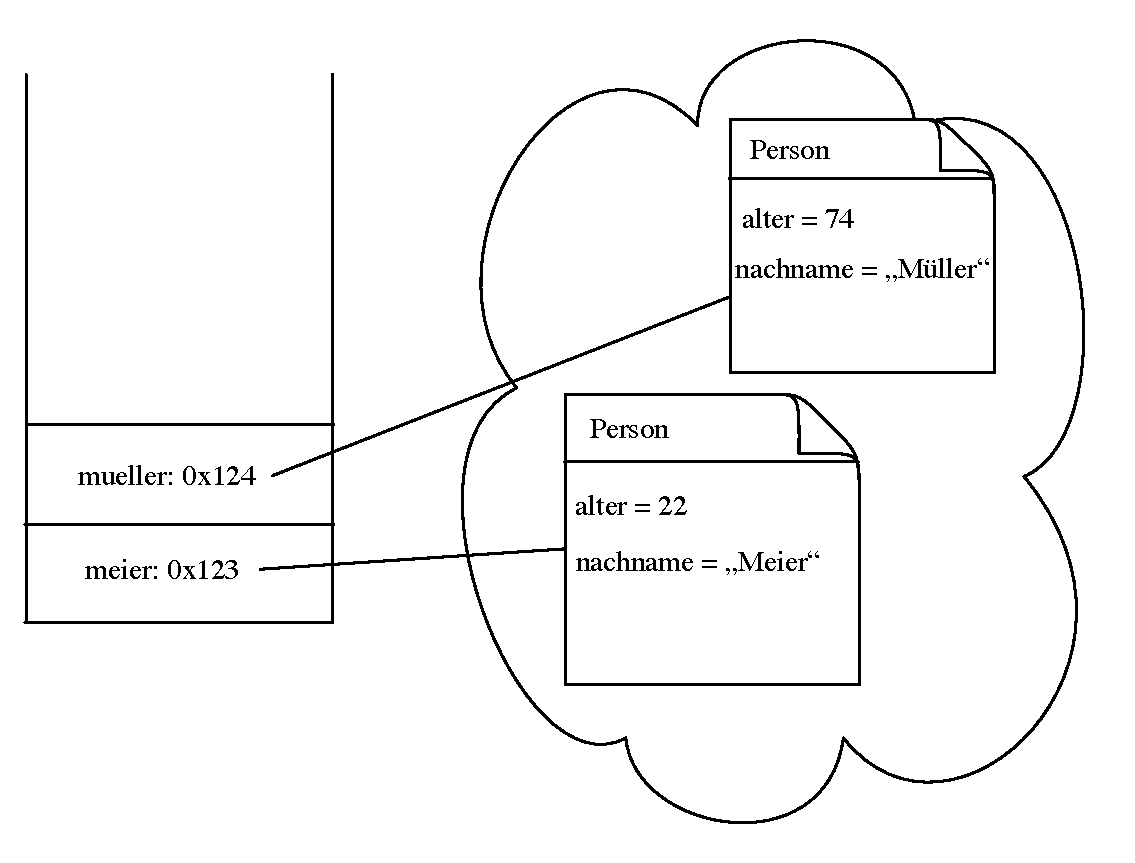
\includegraphics[width=0.8\textwidth]{stackheap_1}
\label{fig:stackheap1}
\caption{Die Adresse der zwei Objekte liegt auf dem Stack, die zwei Objekte liegen jedoch auf dem Heap.}
\end{figure}

Nun wollen wir das oben angesprochene Konzept erweitern, indem wir die beiden Personen heiraten lassen. Hierzu fügen wir die Funktion \texttt{heiraten(Person person)} auf.

\begin{lstlisting}
Person mueller;

meier = new Person();
meier.alter = 74;
meier.nachname = "Meier";

mueller = new Person();
mueller.alter = 22;
mueller.nachname = "Müller";

meier.heiraten(mueller);
\end{lstlisting}

Durch die Methode heiraten, wird die Adresse des ehepartners in der Variable Ehepartner gespeichert. Diese Adresse zeigt auf das Objekt des ehepartners. Da beide Personen miteinander verheiratet sind, zeigen sie jeweils aufeinander.

\begin{figure}[htbp!] 
\centering    
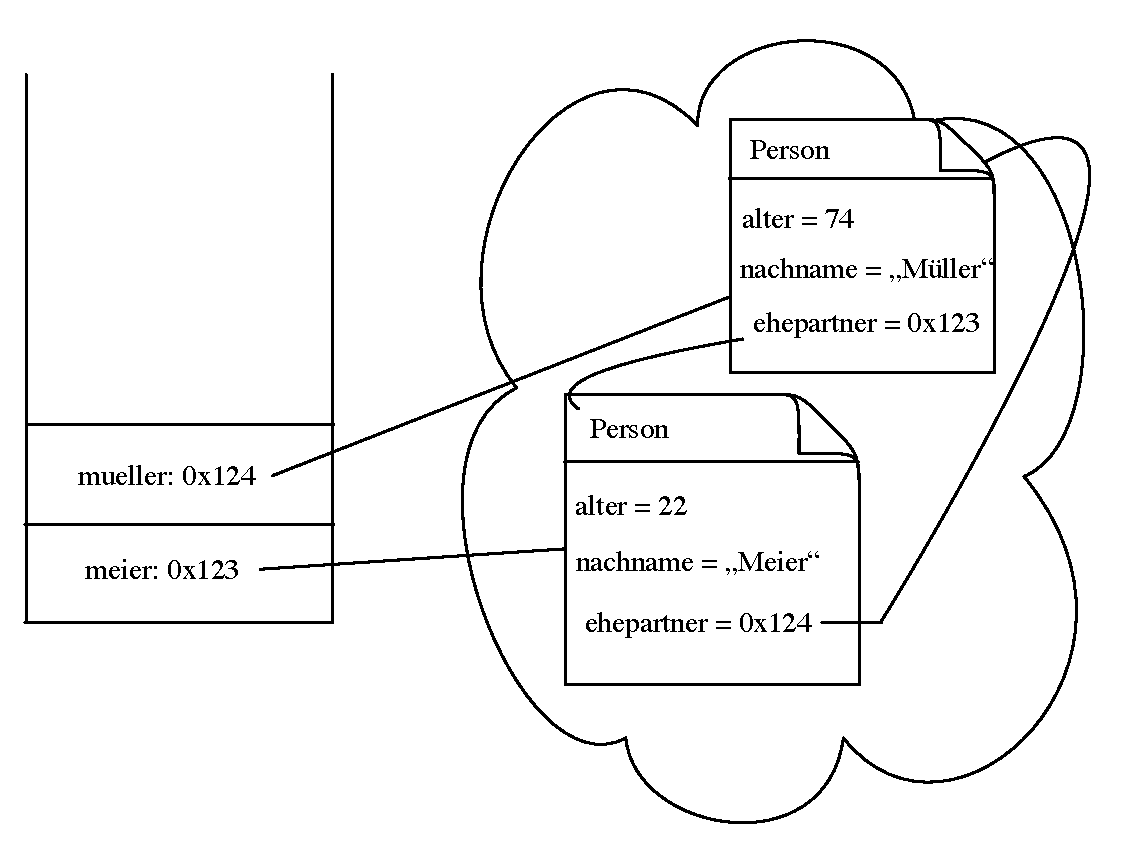
\includegraphics[width=0.8\textwidth]{stackheap_2}
\label{fig:stackheap2}
\caption{Der Stack und Heap nach dem Aufruf der Methode heiraten().}
\end{figure}

Es gilt zu beachten, dass hier die String Literale, die in \texttt{nachname} gespeichert werden, hier vereinfacht wie Instanzvariablen behandelt wurden. In der Realität sind Strings jedoch auch Objekte und somit würde nachname eigentlich auf ein anderes Objekt vom Typ String zeigen, welches dann den Nachnamen darstellt. Ich habe der Anschaulichkeit halber die Strings jedoch wie Instanzvariablen behandelt.

\subsubsection{Garbage Collector}
Ein interessantes Konzept ist das des Garbage Collectors, welches hier nur angeschnitten werden soll. Dieser ist für die Speicherverwaltung auf dem Heap zuständig und sorgt dafür, dass nicht mehr benutzte Objekte aus dem Heap genommen werden, um Speicherplatz zu sparen. Es gibt verschiedene Möglichkeiten, zu bestimmen, welche Objekte wann nicht mehr gebraucht werden, jedoch ist dies ein eigenes Feld für sich und wird eventuell in einer späteren Vorlesung genauer besprochen.

\section{UML}

Die \texttt{Unified Modeling Language} ist eine standardisierte Modellierungssprache, die 1997 aus vielen verschiedenen Modellierungssprachen in der Version 1.0 vereint wurde. Diese Modellierungssprache wird benutzt, um Objekte abstrahiert darzustellen, sodass man ohne die genaue Logik zu verstehen, eine ungefähre Ahnung hat, was ein Programm macht. Das Vereinfachen von komplexeren Abläufen ist also die Grundidee von UML.
Ein Modell ist damit kein exakter Nachbau eines Objektes, sondern eine Vereinfachung, welche das Original beschreibt. Dies bezweckt ein besseres Verständnis des Originals.

Trotz des Teilworts \textit{Language} handelt es sich bei UML um Zeichnungen; diese werden als Diagramme bezeichnet. Es gibt unterschiedliche Arten von Diagrammen, die unterschiedliche Aspekte eines Programms berücksichtigen. Insgesamt gibt es 13 verschiedene Diagrammtypen, die entweder \texttt{Strukturdiagramme} sind, oder aber \texttt{Verhaltensdiagramme}. Strukturdiagramme sind (wer hätte es gedacht) Modelle einer Struktur und somit auch statisch. Hier werden Zusammenhänge beschrieben, was wir im Folgenden anhand der \texttt{Klassendiagramme} zeigen werden. Verhaltensdiagramme erklären die Abläufe eines Programms und sind aus diesem Grund dynamisch. \texttt{Aktivitätsdiagramme} zählen zu den Verhaltensdiagrammen.

\section{Aktivitätsdiagramme}

Aktivitätsdiagramme beschreiben den Ablauf, wie ein Programm funktioniert, besonders die Eigenschaft, dass die Reihenfolge dargestellt wird ist teilweise sehr praktisch, um nachzuvollziehen, was ein Programm macht. Prinzipiell kennt ein Aktivitätsdiagramm nur zwei Arten von Bausteinen. Knoten und Kanten. Knoten sind die Stellen, an denen etwas passiert, und werden deshalb auch als \texttt{Aktivitäten} bezeichnet; Kanten verbinden diese Aktivitäten miteinander. Es gibt zudem noch Startknoten und Endknoten. \underline{Wichtig:} Es ist zwar unüblich, dass mehrere Start- und/oder Endknoten vorkommen, aber dies ist nicht verboten.

Wie der Name es schon impliziert, beginnt eine Prozedur bei einem Startknoten. Man kann sich vorstellen, dass ein \texttt{Token} von dort aus über die Kanten zu den einzelnen Knoten fährt, dort eine Aktion ausgeführt wird und das Token im Anschluss weiterfährt, bis es zu einem Endknoten gelangt.

Wir möchten uns nun angucken, wie ein solches Aktivitätsdiagramm aussieht.

\subsubsection{Beispiel}

\begin{mpost}[mpsettings={input metauml;},use]
Begin.b;
Activity.eat("Esse Etwas");
Branch.enough;
Fork.fork("h", 50);
Activity.read("Lies ein Buch");
Activity.listen("Musik hören", "(im Hintergrund)");
Fork.join("h", 50);
End.e;

leftToRight.top(10)(read, listen);
Group.readListen(read, listen);

leftToRight(30)(b, eat);
topToBottom(20)(eat, enough, fork, readListen, join, e);

drawObjects(b, eat, enough, fork, readListen, join, e);

clink(transition)(b, eat);
clink(transition)(eat, enough);
link(transition)(pathStepX(enough.e, eat.e, 80));
clink(transition)(enough, fork);
clink(transition)(fork, read);
clink(transition)(fork, listen);
clink(transition)(read, join);
clink(transition)(listen, join);
clink(transition)(join, e);

item(iGuard)("[noch hungrig]")(obj.sw = enough.e + (20, 0));
item(iGuard)("[satt]")(obj.nw = enough.s + (0, -4));
  	  
\end{mpost}

Das oben abgebildete Diagramm beinhaltet alle wichtigen Komponenten, die nötig sind, wenn man einen Ablauf beschreibt. Es ist schnell erkenntlich, was dort dargestellt wird. Man isst etwas. Es wird geprüft, ob man satt ist, ist dies nicht der Fall, isst man so lange weiter, bis man satt ist. Im Anschluss liest man ein Buch und \underline{parallel} dazu hört man Musik. Außerdem sieht man hier, wie die Knoten und Kanten aussehen. Wir wollen jetzt etwas genauer auf die verschiedenen Objekte eingehen.

\subsection{Start- und Endknoten}

Es muss für einen Menschen, der sich mit dem Programm, bzw. der Prozedur noch gar nicht auskennt, schnell ersichtlich sein, wo ein Programm beginnt und wann dieses beendet ist. Dazu sind spezielle Knoten wichtig, die unten abgebildet sind. Der ausgefüllte Knoten ist ein Startknoten, der ausgefüllte Knoten mit dem Kreis drum, ist ein Endknoten.\\

\begin{mpost}[mpsettings={input metauml;},use]
Begin.b;
End.e;
leftToRight(20)(b, e);
drawObjects(b, e);
\end{mpost}

\subsection{Aktionen}

Aktionen werden durch Knoten mit einem rechteckigen Kasten und abgerundeten Ecken dargestellt. Darin steht kurz und knapp, welche Aktion bei diesem Knoten ausgeführt wird. Es ist eventuell sinnvoll, sich vorzustellen, dass jede Aktion der Aufruf einer Funktion im Programm ist.\\


\begin{mpost}[mpsettings={input metauml;},use]
Activity.A("Male Aktivitätsdiagramm");
drawObject(A);
\end{mpost}

\subsection{Verzweigungen}
Verzweigungen sind sinnvoll, um ein komplexeres Programm zu schreiben. Im Beispiel oben soll beispielsweise so lange gegessen werden, bis man satt ist. Somit gibt es nach der Aktion essen zwei Möglichkeiten: Weiter essen, oder zur nächsten Aktion springen. Bereits die Fomulierung ähnelt sehr stark einer Schleife aus der Programmierung. 

\begin{lstlisting}
do {
	nimmNahrungAuf();
} while (hungrig());
\end{lstlisting}

Dies entspricht diesem Aktivitätsdiagramm: \\

\begin{mpost}[mpsettings={input metauml;},use]
Begin.b;
Activity.eat("Esse Etwas");
Branch.enough;
End.e;

leftToRight(30)(b, eat);
topToBottom(20)(eat, enough, e);

drawObjects(b, eat, enough,e);

clink(transition)(b, eat);
clink(transition)(eat, enough);
link(transition)(pathStepX(enough.e, eat.e, 80));
clink(transition)(enough, e);

item(iGuard)("[noch hungrig]")(obj.sw = enough.e + (20, 0));
item(iGuard)("[satt]")(obj.nw = enough.s + (0, -4));
\end{mpost}

Nehmen wir nochmal das Token, das über die Kanten zu den verschiedenen Knoten fährt. Dann nimmt dieses Nahrung auf, fährt zu der Verzweigung und es wird geguckt, ob genug Nahrung aufgenommen wird. An den ausgehenden Kanten sieht man, welche der jeweiligen Wege das Token einschlagen wird, da dort (in eckigen Klammern) die Bedingung zum weiterfahren steht. Somit hat es etwas von einem if statement, welches true, oder false zurückgibt. Somit sind sowohl sehr unterschiedliche Wege möglich und im speziellen, wie im Beispiel, Schleifen.
Verzweigungen führen jedoch nicht immer nur verschiedene Kanten in verschiedene Richtungen, sie werden auch genutzt um unterschiedliche Pfade zusammen zu führen. 

\subsection{Gabelungen}

Bei Verzweigungen wird ja das Token nur auf eine der ausgehenden Kantenlinien weitergeleitet. Möchte man jedoch bestimmte Schritte nebeneinander ausführen (Stichwort: Multitasking), so sind \texttt{Gabelungen} nötig. Hier wird das Token kopiert und nimmt jede der möglichen Ausgangskanten. 
Dies sieht dann so aus: \\

\begin{mpost}[mpsettings={input metauml;},use]
Begin.b;
Fork.fork("h", 50);
Activity.read("Lies ein Buch");
Activity.listen("Musik hören");
Fork.join("h", 50);
End.e;

leftToRight.top(10)(read, listen);
Group.readListen(read, listen);

topToBottom(20)(b, fork, readListen, join, e);

drawObjects(b, fork, readListen, join, e);

clink(transition)(b, fork);
clink(transition)(fork, read);
clink(transition)(fork, listen);
clink(transition)(read, join);
clink(transition)(listen, join);
clink(transition)(join, e);
\end{mpost}

Bei diesem Aktivitätsdiagramm wird zur selben Zeit gelesen und Musik gehört. Am Ende, wenn Beides beendet ist, terminiert das Programm. Es ist sehr wichtig zu beachten, dass beim zusammenführen auf die anderen noch laufenden Prozesse gewartet wird. Erst wenn alle Aktionen abgeschlossen sind und bei der Gabelung (die die Kanten wieder zusammen fasst) eintreffen, läuft das Programm weiter.

Nehmen wir als Beispiel den Boxenstopp eines Rennautos: Das Auto fährt in die Boxengasse und ab dem Zeitpunkt wo es hält, werden unterschiedliche Aktionen (parallel) ausgeführt: Die Reifen werden gewechselt, das Rennauto wird betankt, das Visier des Rennfahrers wird eventuell geputzt usw. Der Rennfahrer darf aber erst weiterfahren, wenn alle diese Aktionen abgeschlossen sind, sonst steckt eventuell noch der Tankrüssel im Wagen.

\section{Klassendiagramme}

\texttt{Klassendiagramme} werden dazu benutzt um den Aufbau von Klassen zu beschreiben und die Zusammenhänge zwischen einzelnen Klassen darzustellen. Es ist sehr praktisch objektorientierte Projekte anhand dieser Klassendiagramme zu planen, da man die einzelnen Eigenschaften der Objekte sehr schön darstellen kann und somit einen engen Bezug zur Wirklichkeit hat. Aber bevor wir auf diese Eigenschaften näher eingehen wollen, möchten wir uns erst einmal die Beziehungen zwischen den Klassen ansehen.

\subsection{Assoziation}
\begin{mpost}[mpsettings={input metauml;},use]
Class.A("Klasse A")()();

Class.B("Klasse B")()();

leftToRight(100)(A, B);
drawObjects(A, B);

link(associationUni)(A.e -- B.w);
\end{mpost}\\

Die Verbindungslinie zwischen der \texttt{Klasse A} zu der \texttt{Klasse B} bedeutet, dass \texttt{Klasse A} auf \texttt{Klasse B} zugreifen kann. Die Pfeilrichtung gibt an, welche Klasse auf wen Zugriff hat, es ist auch möglich, dass beiden Klassen aufeinander zugreifen, dann ist an beiden Enden der Verbindungslinie ein Pfeil. Es ist auch möglich die Pfeilspitzen wegzulassen, das ist bei unwichtigen Beziehungen teilweise der Fall.


\subsection{Komposition}
\begin{mpost}[mpsettings={input metauml;},use]
Class.C("Klasse C")()();

Class.D("Klasse D")()();

leftToRight(100)(C, D);
drawObjects(C, D);

link(composition)(C.e -- D.w);
\end{mpost}\\

Hier ist eine \texttt{Komposition} dargestellt. Eine Komposition bedeutet, dass eine Klasse ohne eine andere Klasse nicht auskommt. Die Raute befindet sich an dem Ende der Verbindungslinie, an dem die abhängige Klasse steht. Nehmen wir als Beispiel die Klassen Mensch und Erde. Ein Mensch muss auf der Erde leben, die Erde kann aber auch ohne Menschen auskommen.

\subsection{Vererbung}
\begin{mpost}[mpsettings={input metauml;},use]
Class.E("Klasse E")()();

Class.F("Klasse F")()();

leftToRight(100)(E, F);
drawObjects(E, F);

link(inheritance)(E.e -- F.w);
\end{mpost}\\

Der Vollständigkeit halber soll hier auch einmal die Beziehung im Sinne der Vererbung gezeigt werden. Da Vererbung aber noch nicht in der Vorlesung besprochen wurde, wird hierauf im Weiteren nicht näher eingegangen.

\subsection{Assoziationen verfeinern}

Oben haben wir gesehen, dass man beschreiben kann, ob eine Klasse von einer Anderen abhängig ist. Möchte man jedoch genauer sagen, in welchem Maße diese Abhängigkeit steht, kann man sog. \texttt{Multiplizitäten} angeben. Es gibt \texttt{1:1}, \texttt{1:n} und \texttt{n:n} Beziehungen. Steht keine genauere Angabe an den Verbindunglinien, wird von einer 1:1 Beziehung ausgegangen. Das bedeutet, dass jedes Objekt einer Klasse mit genau einem Objekt der anderen Klasse in Kontakt steht. Eine 1:n Beziehung wird angegeben, wenn ein Objekt einer Klasse mit mehreren Objekten einer anderen Klasse in Kontakt steht. Somit ist auch klar, dass eine n:n Beziehung aussagt, dass Objekte beider Klassen Zugriff auf mehrere Objekte der anderen Klasse haben. Wie bereits beschrieben, muss man 1:1 Beziehungen nicht explizit angeben. Um eine 1:n Beziehung darzustellen, schreibt man ein 0..* an das navigierbare Ende. 0..* liest man wie $n \in N_{0}$.\\

\begin{mpost}[mpsettings={input metauml;},use]
Class.A("Klasse A")()();

Class.B("Klasse B")()();

leftToRight(100)(A, B);
drawObjects(A, B);

link(associationUni)(A.e -- B.w);
item(iAssoc)("0..*")(obj.n  = .8[A.e,B.w]);

\end{mpost}\\

Man kann somit aber auch Ober- und Untergrenzen festlegen, also beispielsweise 2..5 (mindestens 2, aber maximal 5).

\subsection{Klassen beschreiben}

Eine Klasse ist ein Rechteck und hat drei Unterbereiche, welche oben bisher leer gelassen wurden. So gibt es den \texttt{Klassennamen}, darunter befinden sich die \texttt{Eigenschaften} und im letzten Unterbereich befinden sich die \texttt{Methoden}. 
%Um möglichst nah an der Objektorientierung zu sein, kann man den Eigenschaften und Methoden auch eine Sichtbarkeit zuordnen, so schreibt man für \texttt{private} ein - (Minuszeichen), für \texttt{public} ein + (Plus) und für \texttt{protected} ein # (Hash-Zeichen). Ein \texttt{Package} kann man über das \tilde (Tildezeichen) definieren. 

Eigenschaften beschreibt man, indem man den Namen angibt, danach kommt ein Doppelpunkt und zuletzt der Datentyp. Bei den Methoden sieht es fast genau so aus, hier kommt zuerst der Methodenkopf und nach dem Doppelpunkt dann der Rückgabewert. Wie bei Java auch, benutzt man bei Klassendiagrammen \texttt{void}, falls man keinen Wert zurück gibt. Hier ist eine Beispielklasse mit verschiedenen Eigenschaften und einer Methode.\\

\begin{mpost}[mpsettings={input metauml;},use]
Class.Person("Person")
		("-alter: int",
		 "-vorname: String",
		 "-nachname: String",
		 "-alter: int"
		 "-freunde: Person 0..*")
		("+heiraten(partner: Person): void",
		 "+sagHallo(): String");

Person.nw = (0, 0);
drawObject(Person);
\end{mpost}\\

Hier haben wir eine Klasse \texttt{Person} mit den privaten Eigenschaften \texttt{vorname} und \texttt{nachname} vom Typ \texttt{String}, der Eigenschaft \texttt{alter} vom Typ int und eine Liste von \texttt{Personen}, die als \texttt{freunde} bezeichnet werden. Alle diese Eigenschaften sind private, bei dem hier benutzten Programm wird dafür ein Schloss verwendet, jedoch ist es üblicherweise einfach ein - (Minuszeichen).

Zudem besitzt diese Klasse zwei Methoden, die beide \texttt{public} sind. Die Methode \texttt{heiraten()}, die den Rückhabewert void hat (also nichts zurück gibt), nimmt einen Parameter \texttt{partner}, der vom Typ \texttt{Person}, entgegen. Und die Methode \texttt{sagHallo()} gibt einen String zurück.

Man sieht, dass die Klassendiagramme einen guten ersten Eindruck über Klassen geben und man die Logik die hinter den einzelnen Methoden steht, nicht unbedingt verstehen muss.

%\include{Chapter4/chapter4}
%\include{Chapter5/chapter5}
%\include{Chapter6/chapter6}
%\include{Chapter7/chapter7}



% ********************************** Back Matter *******************************
% Backmatter should be commented out, if you are using appendices after References
%\backmatter 

% ********************************** Bibliography ******************************
\begin{spacing}{0.9}

% To use the conventional natbib style referencing
% Bibliography style previews: http://nodonn.tipido.net/bibstyle.php

\bibliographystyle{apalike}
%\bibliographystyle{plainnat} % use this to have URLs listed in References
\cleardoublepage
\bibliography{References/references} % Path to your References.bib file


% If you would like to use BibLaTeX for your references, pass `custombib' as 
% an option in the document class. The location of 'reference.bib' should be 
% specified in the preamble.tex file in the custombib section. 
% Comment out the lines related to natbib above and uncomment the following line.

% \printbibliography[heading=bibintoc, title={References}]


\end{spacing}

% *************************************** Index ********************************
\printthesisindex % If index is present

\end{document}
